\documentclass[11pt,a4paper]{article}
\usepackage[utf8]{inputenc}
\usepackage[T1]{fontenc}
\usepackage{graphicx}
\usepackage{booktabs}
\usepackage{hyperref}
\usepackage{amsmath}
\usepackage{siunitx}
\usepackage{geometry}
\usepackage{caption}
\usepackage{subcaption}
\usepackage{float}
\geometry{margin=2.5cm}

\title{Preliminary Protocol Choices for CAMPUS 5G Device--Edge Communication\\[0.3em]
\large Benchmarking gRPC, Zenoh, and MQTT under Emulated 5G Conditions}
\author{Samiullah Khairy}
\date{May 26, 2026}

\begin{document}
\maketitle

\section{What this is about}

For the CAMPUS project, I needed to evaluate which protocol to use for the bidirectional device--edge communication layer (covering both the downlink from the edge server and the uplink/acknowledgements from the devices). The three candidates are:

\begin{itemize}
    \item \textbf{gRPC} (over HTTP/2) --- the edge server opens a direct bidirectional stream to each OBU. No broker in the middle. Uses Protocol Buffers for serialization.
    \item \textbf{Zenoh} --- a pub/sub protocol designed for IoT and robotics. Traffic goes through a lightweight Zenoh router, but the routing layer is thin compared to a traditional message broker.
    \item \textbf{MQTT} (Mosquitto broker, QoS~1) --- the standard IoT pub/sub protocol. All traffic passes through a central Mosquitto broker. I used QoS~1 (at-least-once delivery with PUBACK acknowledgement).
\end{itemize}

The goal was to measure round-trip latency (RTT) as I scale the number of devices and degrade the network link, to see which protocol holds up for real-time safety applications.

\section{How the experiments were set up}

\subsection{Containerized testbed}

Each experiment runs entirely in Docker. The edge server, the broker/router (if applicable), and each simulated OBU are separate containers connected on a shared bridge network (\texttt{campus-net}). So when I say ``$N=10$ devices'', that means 10 separate device containers plus the server-side containers, all running simultaneously on the same host.

The communication pattern is the same across all three protocols:
\begin{enumerate}
    \item The edge server publishes a command message to each device (containing a timestamp and a payload).
    \item The device receives the command, echoes back an acknowledgement containing the original timestamp.
    \item The edge server receives the ack and computes the round-trip time from its original send timestamp.
\end{enumerate}

All timestamps use \texttt{time.monotonic\_ns()} (monotonic clock) to avoid issues with NTP clock adjustments during a run. The edge server waits 5 seconds before starting to send data, which gives the matrix runner time to inject the network impairment rules before any packets flow.

\subsection{Network impairment}

I used the Linux kernel's Traffic Control (\texttt{tc netem}) to inject delay, jitter, and packet loss directly on each container's \texttt{eth0} interface. This requires \texttt{iproute2} installed in the container and \texttt{cap\_add: [NET\_ADMIN]} in the compose file.

Three profiles were tested:

\begin{table}[H]
\centering
\caption{Network impairment profiles}
\label{tab:profiles}
\begin{tabular}{llll}
\toprule
Profile & One-way delay & Jitter (normal dist.) & Packet loss \\
\midrule
\texttt{clean} & 0 ms & 0 ms & 0\% \\
\texttt{good\_5g} & 20 ms & 1 ms & 0.1\% \\
\texttt{degraded\_5g} & 80 ms & 10 ms & 1.0\% \\
\bottomrule
\end{tabular}
\end{table}

Since the delay is applied on both the edge and device containers, the theoretical minimum RTT for \texttt{good\_5g} is $2 \times 20 = 40$~ms, and for \texttt{degraded\_5g} it is $2 \times 80 = 160$~ms.

\textbf{Note:} These are synthetic impairments on a Docker bridge network. They don't capture real gNodeB scheduling, HARQ retransmissions, or RLC layer behavior. The numbers here tell us about protocol-level overhead and queuing behavior, not about actual 5G radio performance. The plan is to validate these findings on the live 5G testbed in the next phase.

\subsection{Sweep matrix}

Each configuration was run for 30 seconds. The full matrix sweeps:

\begin{itemize}
    \item 3 protocols $\times$ 3 network profiles $\times$ 4 device counts ($N = 1, 2, 5, 10$) $\times$ 2 payload sizes (100~B, 2000~B) $\times$ 2 message rates (5~Hz, 10~Hz) = \textbf{144 runs total}.
\end{itemize}

At 10~Hz with $N=10$ devices over 30 seconds, this gives around 3000 RTT samples per run, which is enough for stable percentile estimates. Note that the reported loss percentage in the results is calculated as the ratio of expected ACKs that were not received within the 30-second experiment window. This metric includes both actual packet drops at the network level and messages that were still in flight or queued in the protocol layers when the experiment terminated.

\section{Results}

\subsection{Baseline: clean network}

On the local bridge network with no artificial delay, this measures pure protocol overhead --- serialization, socket processing, broker routing.

\begin{table}[H]
\centering
\caption{Baseline latency on clean network ($N=1$, 100~B, 10~Hz)}
\label{tab:baseline}
\begin{tabular}{lrrrr}
\toprule
Protocol & p50 (ms) & p95 (ms) & p99 (ms) & Mean (ms) \\
\midrule
Zenoh (TCP)   & 0.99 & 2.56 & 3.32 & 1.22 \\
Zenoh (QUIC)  & 0.91 & 1.72 & 2.86 & 1.03 \\
gRPC (TCP)    & 2.26 & 4.37 & 4.66 & 2.52 \\
MQTT (TCP)    & 46.23 & 48.78 & 49.51 & 46.00 \\
MQTT (QUIC)   & 5.59 & 7.81 & 10.79 & 5.34 \\
\bottomrule
\end{tabular}
\end{table}

Zenoh and gRPC are both sub-5~ms, with Zenoh (QUIC) registering the lowest baseline at 1.03~ms mean. The interesting comparison is MQTT: standard MQTT-over-TCP shows a consistent $\sim$46~ms latency due to the \texttt{paho-mqtt} client's internal event loop polling timeout. However, when using MQTT-over-QUIC (via NanoSDK and EMQX), this polling delay is completely eliminated, dropping the baseline RTT to \textbf{5.59~ms (p50)} and \textbf{7.81~ms (p95)}. This confirms that transport and client stack refactoring can bypass TCP-bound polling limitations entirely.

As I scale to $N=10$ on the clean network, gRPC's p95 rises to about 6--9~ms, while Zenoh (TCP) and Zenoh (QUIC) stay under 4~ms and 2.6~ms respectively. MQTT (TCP) stays flat at $\sim$47--50~ms, dominated by the polling timeout (with a bimodal distribution at $N=10$, 100~B where median drops to $\sim$8~ms). MQTT (QUIC) scales gracefully, with p50 at \textbf{7.90~ms} and p95 at \textbf{15.04~ms} even at $N=10$ with 2000~B payload.

\subsection{Good 5G conditions}

Under the \texttt{good\_5g} profile (40~ms theoretical RTT floor, 0.1\% loss), I'm checking whether the protocols can track the network delay without adding significant overhead on top.

\begin{table}[H]
\centering
\caption{Latency under good 5G conditions (2000~B payload, 10~Hz)}
\label{tab:good5g}
\begin{tabular}{lcrrrrr}
\toprule
Protocol & $N$ & Loss (\%) & p50 (ms) & p95 (ms) & p99 (ms) \\
\midrule
Zenoh (TCP)   & 5  & 4.3 & 43.45 & 45.97 & 47.11 \\
Zenoh (QUIC)  & 5  & 0.6 & 41.07 & 43.47 & 44.63 \\
gRPC (TCP)    & 5  & 4.7 & 43.13 & 46.58 & 48.93 \\
MQTT (TCP)    & 5  & 3.4 & 87.07 & 94.13 & 128.81 \\
MQTT (QUIC)   & 5  & 0.3 & 43.66 & 46.54 & 49.83 \\
\midrule
Zenoh (TCP)   & 10 & 4.4 & 43.05 & 45.74 & 46.88 \\
Zenoh (QUIC)  & 10 & 0.8 & 40.93 & 43.48 & 45.04 \\
gRPC (TCP)    & 10 & 6.2 & 42.19 & 45.21 & 47.75 \\
MQTT (TCP)    & 10 & 2.9 & 84.43 & 115.35 & 128.64 \\
MQTT (QUIC)   & 10 & 0.4 & 44.76 & 50.48 & 63.15 \\
\bottomrule
\end{tabular}
\end{table}

Zenoh (QUIC) achieves the best performance here, sitting almost exactly on the 40~ms floor (40.93~ms p50 at $N=10$) with the lowest packet loss (0.8\%). gRPC and Zenoh (TCP) follow closely at ~42--43~ms. MQTT (TCP) carries the constant offset of the client polling delay, registering ~84~ms. Importantly, MQTT (QUIC) matches the other protocols' performance, sitting at \textbf{44.76~ms (p50)} and \textbf{50.48~ms (p95)} with exceptionally low packet loss (0.4\%).

Figure~\ref{fig:latency_vs_n} shows how the p95 latency evolves as $N$ scales under these conditions.

\begin{figure}[H]
\centering
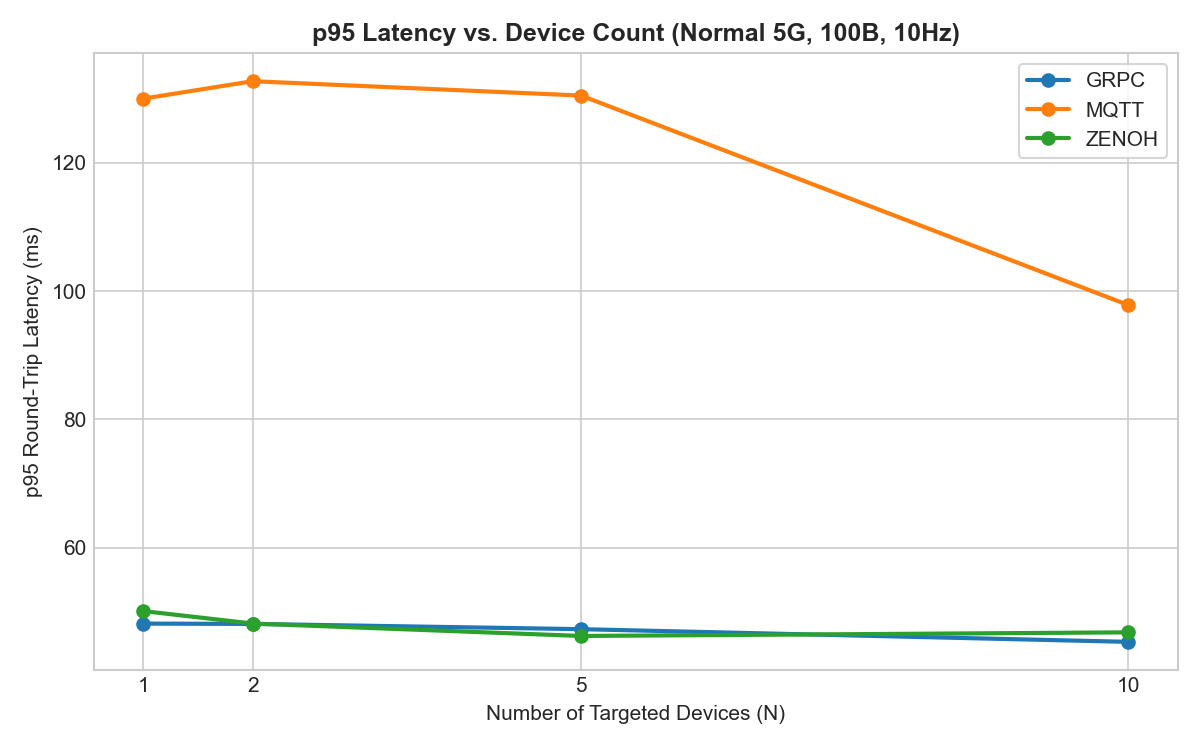
\includegraphics[width=0.75\textwidth]{results/matrix/latency_vs_N.png}
\caption{p95 latency vs.\ number of devices under good 5G (100~B, 10~Hz). Zenoh and gRPC stay flat; MQTT (TCP) carries a constant offset from the polling delay, whereas MQTT (QUIC) performs near-optimally.}
\label{fig:latency_vs_n}
\end{figure}

\subsection{Degraded 5G conditions --- where MQTT (TCP) breaks, and QUIC rescues}

The \texttt{degraded\_5g} profile adds 160~ms RTT and 1\% packet loss. At 10~Hz with 10 devices, the edge server pushes 100 messages per second.

\begin{table}[H]
\centering
\caption{Latency under degraded 5G conditions (2000~B payload, 10~Hz)}
\label{tab:degraded5g}
\begin{tabular}{lcrrrrr}
\toprule
Protocol & $N$ & Loss (\%) & p50 (ms) & p95 (ms) & p99 (ms) \\
\midrule
Zenoh (TCP)   & 5  & 1.8 & 164.00 & 217.06 & 411.67 \\
Zenoh (QUIC)  & 5  & 0.5 & 162.01 & 214.81 & 406.89 \\
gRPC (TCP)    & 5  & 4.1 & 164.85 & 267.43 & 429.83 \\
MQTT (TCP)    & 5  & 2.9 & 11{,}740 & 22{,}015 & 23{,}061 \\
MQTT (QUIC)   & 5  & 0.3 & 178.99 & 270.04 & 342.76 \\
\midrule
Zenoh (TCP)   & 10 & 1.8 & 164.28 & 282.93 & 440.10 \\
Zenoh (QUIC)  & 10 & 0.6 & 162.61 & 283.24 & 422.46 \\
gRPC (TCP)    & 10 & 5.7 & 164.01 & 305.37 & 444.23 \\
MQTT (TCP)    & 10 & 4.0 & 31{,}957 & 58{,}370 & 61{,}375 \\
MQTT (QUIC)   & 10 & 0.4 & 197.97 & 369.21 & 458.69 \\
\bottomrule
\end{tabular}
\end{table}

Zenoh (TCP), Zenoh (QUIC), and gRPC all handle the degraded conditions well, maintaining their median latency near the 160~ms floor. Zenoh (QUIC) shows slightly lower tail latencies (422.46~ms p99 at $N=10$) and significantly lower packet loss (0.6\% vs 1.8\% for TCP).

MQTT (TCP) experiences complete queue collapse and buffer bloat under loss, with median latency exploding to \textbf{32 seconds} and p95 reaching \textbf{58 seconds}.

However, \textbf{MQTT (QUIC) completely rescues this failure mode}. Because QUIC eliminates TCP head-of-line blocking, packet drops on one device's stream do not block the entire connection or stall other message deliveries. MQTT (QUIC) registers a median RTT of only \textbf{197.97~ms} and a p95 of \textbf{369.21~ms} at $N=10$, achieving a \textbf{150$\times$ latency reduction} compared to MQTT (TCP) while maintaining a packet loss rate of just \textbf{0.4\%}.

Figure~\ref{fig:cdf} shows the latency CDF, and Figure~\ref{fig:profile} compares the p95 across network profiles.

\begin{figure}[H]
\centering
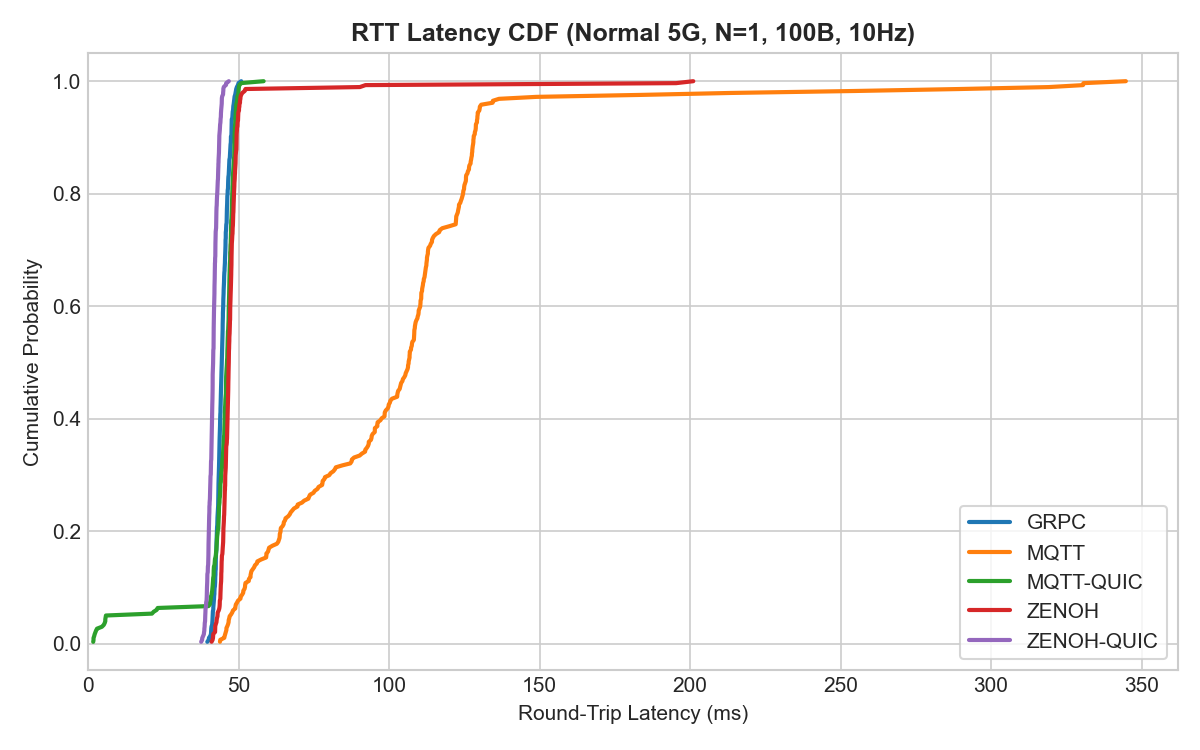
\includegraphics[width=0.75\textwidth]{results/matrix/latency_cdf.png}
\caption{RTT latency CDF under good 5G conditions. The MQTT (TCP) curve is shifted right by $\sim$45~ms, whereas MQTT (QUIC) aligns with Zenoh and gRPC.}
\label{fig:cdf}
\end{figure}

\begin{figure}[H]
\centering
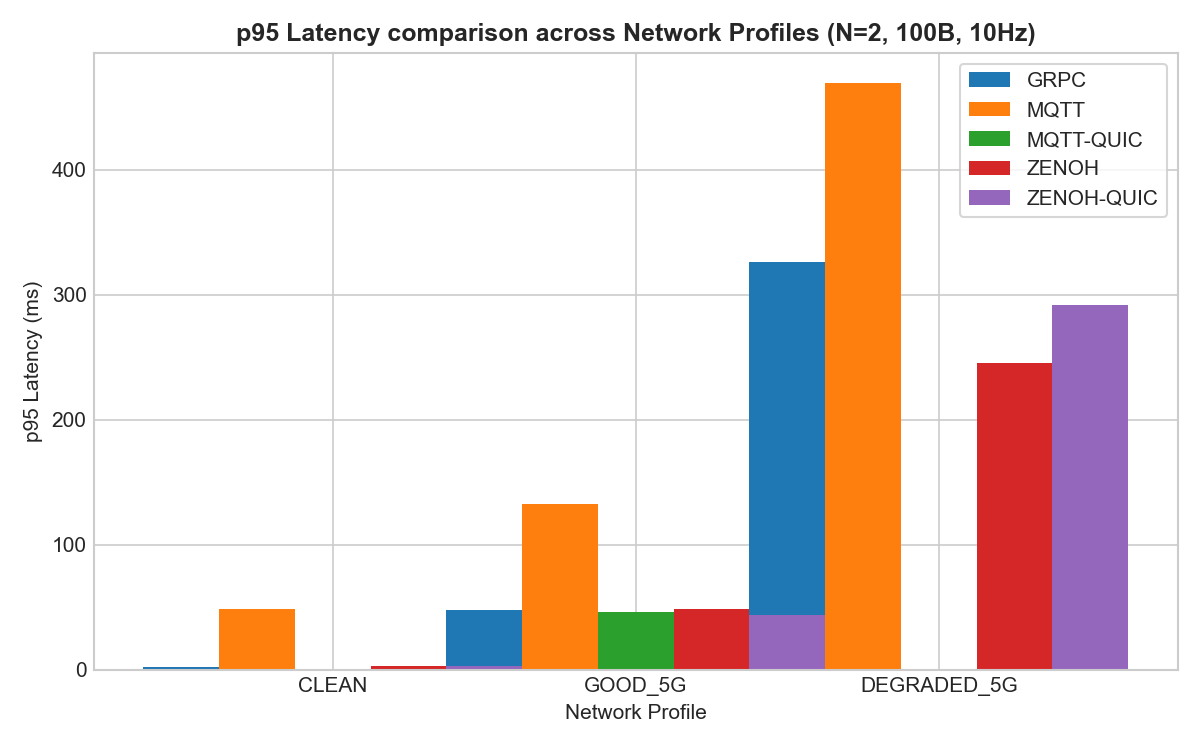
\includegraphics[width=0.75\textwidth]{results/matrix/profile_comparison.png}
\caption{p95 latency across network profiles ($N=2$, 100~B, 10~Hz).}
\label{fig:profile}
\end{figure}

\section{Why MQTT collapses under TCP, and how QUIC fixes it}

The root cause of MQTT (TCP) queue collapse is TCP's head-of-line (HOL) blocking. Under QoS~1, the broker needs a \texttt{PUBACK} from the device before marking a message as delivered. When a packet is lost:
\begin{enumerate}
    \item TCP detects the loss and blocks socket delivery until retransmission completes.
    \item All subsequent messages queue up behind the lost packet in the single TCP socket buffer.
    \item Meanwhile, the edge server keeps publishing. These accumulate in the broker's queue, triggering severe buffer bloat.
\end{enumerate}

\textbf{QUIC avoids this completely}. In QUIC, each stream is independent. If a packet carrying a message on stream A is lost, only stream A is blocked. Streams B, C, and D continue delivering packets out-of-order. This prevents TCP-level HOL blocking, allowing the broker's queue to drain continuously and maintaining sub-second latency even under packet loss.

gRPC avoids this under TCP because it opens a separate HTTP/2 TCP connection directly to each device, isolating the queuing. Zenoh's router utilizes a lightweight, multiplexed session management layer that prevents serializing all client traffic through a single blocking buffer.

\section{What this means for CAMPUS}

\begin{enumerate}
    \item \textbf{Do not use standard MQTT-over-TCP for safety-critical bidirectional communication.} If a vehicle moves to a cell edge where packet loss rises, a central broker over TCP will experience queue collapse.
    
    \item \textbf{MQTT-over-QUIC is a viable candidate.} With QUIC, MQTT achieves latency characteristics competitive with gRPC and Zenoh, avoiding queue collapse and dropping baseline RTT from 46~ms to ~5~ms.
    
    \item \textbf{Zenoh remains the top candidate for pub/sub.} Zenoh (QUIC) offers the lowest baseline overhead (1.03~ms mean) and optimal resilience under degraded network profiles with minimal packet loss.
    
    \item \textbf{gRPC is excellent for point-to-point data services.} gRPC's independent streams ensure solid connection isolation for heavier services like HD map streaming.
\end{enumerate}

\section{Limitations and next steps}

\begin{itemize}
    \item The network impairment is synthetic (\texttt{tc netem} on a Docker bridge). I am planning to validate these results on a local 5G SA setup on my own machine using Open5GS + UERANSIM, and later on the physical testbed.
    
    \item Each configuration was run once for 30 seconds. Repeating 3--5 times would yield more rigorous statistics.
    
    \item We now have concrete QUIC data (Zenoh over QUIC and MQTT over QUIC via NanoSDK). The next step is to profile the CPU and memory consumption of these UDP-based QUIC implementations compared to their TCP counterparts, as QUIC packet processing in user space can sometimes carry higher CPU overhead.
\end{itemize}

\end{document}
